% вторая часть

\section{Архитектура и проектирование модулей системы}

\subsection{Общая архитектура системы и сценарий работы}
Система реализована как веб-приложение на фреймворке Django~\cite{django2026docs}
и включает шесть функциональных модулей: управление пользователями, 
учебный контент, адаптивная система обучения с контекстной адаптацией. 
Взаимодействие между модулями построено по принципу слабой 
связанности через сигнальный механизм Django, что обеспечивает 
независимое тестирование и масштабирование компонентов~\cite{gamma1994design}.

Полный сценарий работы системы с пользователем включает шесть этапов:
\begin{itemize}
    \item Регистрация. Студент вводит регистрационные данные. 
    Система создаёт пользовательский слот, инициализирует с нулевым счётом баллов
    и запускает фоновое определение геолокации по IP-адресу~\cite{ipapi2026} и собирает данные по 
    движению мыши.
    
    \item Психологическое тестирование. 
    Студент проходит тестирование по психологическим факторам A1–A4. 
    Система генерирует персонализированный набор тестов, 
    обрабатывает ответы и формирует когнитивный профиль с 
    тремя типами рекомендаций (T, R, C)~\cite{brusilovsky2007usermodels, conati2002bayesian}.
    
    \item Выдача первоначальной рекомендации обучения. 
    Модуль рекомендаций синтезирует данные когнитивного профиля, данные поведения
    мыши и текущее значение параметра~$P$ для формирования индивидуального 
    плана на семестр или курс~\cite{brusilovsky2007usermodels, ifenthaler2020learning}.
    
    \item Обучение с контрольными точками. Студент проходит курс по адаптивной 
    траектории, при необходимости скорректированной преподавателем. В заданных 
    преподавателем контрольных точках система генерирует тесты по пройденному 
    материалу, обновляет текущую модель знаний и пересчитывает параметр~$P$~\cite{vanlehn2006behavior, woolf2009building}.
    
    \item Модификация стратегии. На основе обновлённых данных
    система корректирует план обучения. Модуль игровой адаптации начисляет баллы 
    за прохождение контрольных точек в зависимости от успехов обучающегося~\cite{dominguez2013gamifying, plass2015foundations, bartle1996players}.
    
    \item Прогноз и наставнические рекомендации. На основе итогов текущего 
    курса система прогнозирует успеваемость по курсам со схожими компетенциями 
    и формирует рекомендации по построению дальнейшей образовательной траектории~\cite{ifenthaler2020learning}.
\end{itemize}

Взаимодействие модулей согласно этим этапам наглядно показано на схеме ниже.
\begin{figure}[H]
\centering

\includegraphics[width=1\linewidth]{pics/rel} % изображения хранятся в подкаталоге pics
\caption{Схема взаимодействия модулей системы}
\label{fig:modules}
\end{figure}

\subsection{Модуль построения профиля обучающегося}
Модуль построения портрета обучающегося является ключевым компонентом 
адаптивной системы~\cite{brusilovsky2007usermodels}. Он отвечает за сбор данных о психологических характеристиках 
студента, их анализ и формирование рекомендаций для персонализации образовательной 
траектории.

Компонент психологического тестирования проводит тесты, охватывающие следующие 
факторы когнитивного профиля~\cite{brusilovsky2007usermodels}:
\begin{itemize}
    \item A1 (самоорганизация) — способность к планированию и управлению учебным временем;
    \item A2 (мотивация) — уровень внутренней и внешней мотивации к обучению;
    \item A3 (стратегия обучения) — предпочтительные способы усвоения информации (визуальный, аудиальный, кинестетический);
    \item A4 (интегральный показатель) — обобщённая оценка готовности к обучению.
\end{itemize}

Компонент обработки результатов рассчитывает числовое значение каждого фактора, 
определяет уровень (низкий / средний / высокий) и формирует три типа рекомендаций:
для преподавателя (T), по обратной связи (R), для работы в учебном сообществе (C)~\cite{brusilovsky2007usermodels, koper2005learner}.

\subsection{Модуль контекстной адаптации и оценка внешних факторов}
\label{sec:contextual_adaptation}

Контекстная адаптация представляет собой корректировку поведения интеллектуальной обучающей системы (ИОС) на основе информации о внешних условиях функционирования, не зависящих непосредственно от учебного контента. В разрабатываемой системе реализован модуль контекстной адаптации, оценивающий три ключевых параметра: географическое положение, погодные условия и температуру воздуха~\cite{chen2008context, ipapi2026, openweathermap2026}.

Научное обоснование связи погодных условий с когнитивной продуктивностью восходит к исследованиям в области экологической психологии. Эмпирические данные свидетельствуют, что при температуре ниже 13~°C или выше 33~°C наблюдается статистически значимое снижение точности выполнения когнитивных задач и скорости обработки информации~\cite{keller2005warm}. Кроме того, пасмурная и дождливая погода снижает уровень серотонина, что отрицательно сказывается на концентрации внимания и рабочей памяти --- механизм, хорошо изученный в контексте сезонных аффективных расстройств~\cite{keller2005warm}.

Для количественной оценки влияния внешних факторов в системе введён интегральный параметр активности пользователя~$P$, рассчитываемый по формуле:
\begin{equation}
    \label{eq:P}
    P = K_{\text{region}} \cdot K_{\text{temp}} \cdot K_{\text{weather}}
\end{equation}
где $K_{\text{region}}$ --- региональный коэффициент, учитывающий климатические особенности; $K_{\text{weather}}$ --- погодный коэффициент, нормализованный к шкале 0--1; $K_{\text{temp}}$ --- температурный коэффициент, отражающий отклонение от комфортного диапазона.

Значение $K_{\text{temp}}$ вычисляется на основе текущего отклонения температуры с учётом нижней границы устойчивости системы:
\begin{equation}
    \label{eq:Ktemp}
    K_{\text{temp}} = \max\left(0{,}1; \ 1 - \frac{|T_{\text{current}} - T_{\text{comfort}}|}{T_{\text{max.diff}}}\right)
\end{equation}
где:
\begin{itemize}
    \item $T_{\text{comfort}}$ --- комфортная температура (в системе принята за 20~°C);
    \item $T_{\text{current}}$ --- текущая температура воздуха;
    \item $T_{\text{max.diff}}$ --- максимальное допустимое отклонение температуры (13~°C), при котором коэффициент снижается до минимального порогового значения.
\end{itemize}

Выбор диапазона 15--25~°C как комфортного опирается на исследования терморегуляции и умственной работоспособности, а значение $T_{\text{comfort}} = 20$~°C соответствует середине этого диапазона и является стандартным нормативом для учебных помещений согласно ГОСТ 30494-2011. Нижняя граница $K_{\text{temp}} = 0{,}1$ введена намеренно: полное обнуление параметра~$P$ привело бы к отказу рекомендательной системы, что нецелесообразно, поскольку даже в экстремальных условиях ИОС должна функционировать в минимальном режиме~\cite{chen2008context}.

Значения коэффициентов определены на основе анализа психофизиологических исследований. Региональные коэффициенты (таблица~\ref{tab:region}) учитывают адаптацию населения к специфическим климатическим зонам.

\begin{table}[htbp]
\centering
\caption{Региональные коэффициенты $K_{\text{region}}$}
\label{tab:region}
\begin{tabular}{|p{5cm}|c|p{6cm}|}
\hline
\textbf{Регион} & \textbf{$K_{\text{region}}$} & \textbf{Обоснование} \\
\hline
Северная Европа & 1{,}2 & Высокая доля неблагоприятных условий, требующая компенсации \\
\hline
Центральная / Западная Европа & 1{,}1 & Умеренный климат со значимыми сезонными колебаниями \\
\hline
Южная Европа & 1{,}0 & Более мягкий климат, меньше экстремальных погодных явлений \\
\hline
Тропические регионы & 0{,}9 & Стабильные температуры, но высокая влажность и риск экстремальных явлений \\
\hline
\end{tabular}
\end{table}

Погодный коэффициент $K_{\text{weather}}$ (таблица~\ref{tab:weather}) нормализован по текущим метеорологическим условиям. Ясная погода ($K = 1{,}0$) принята за базовый уровень оптимальной концентрации. Облачность ($K = 0{,}9$) незначительно снижает естественную освещённость, влияя на циркадные ритмы. Дождь ($K = 0{,}7$) создаёт акустические помехи и ассоциируется со снижением уровня серотонина~\cite{keller2005warm}. Гроза ($K = 0{,}5$) формирует выраженный стрессовый фон, активирующий симпатическую нервную систему. Снег ($K = 0{,}6$) помимо психологического дискомфорта создаёт практические препятствия, увеличивая когнитивную нагрузку, связанную с логистикой~\cite{chen2008context}.

\begin{table}[htbp]
\centering
\caption{Погодные коэффициенты $K_{\text{weather}}$}
\label{tab:weather}
\begin{tabular}{|p{8cm}|c|}
\hline
\textbf{Погодные условия} & \textbf{$K_{\text{weather}}$} \\
\hline
Ясно & 1{,}0 \\
\hline
Облачно & 0{,}9 \\
\hline
Дождь & 0{,}7 \\
\hline
Снег & 0{,}6 \\
\hline
Гроза & 0{,}5 \\
\hline
\end{tabular}
\end{table}

Архитектура модуля контекстной адаптации обеспечивает надёжный сбор и обработку данных. Взаимодействие компонентов визуализировано на рисунке~\ref{fig:modules}.

\begin{figure}[htbp]
\centering
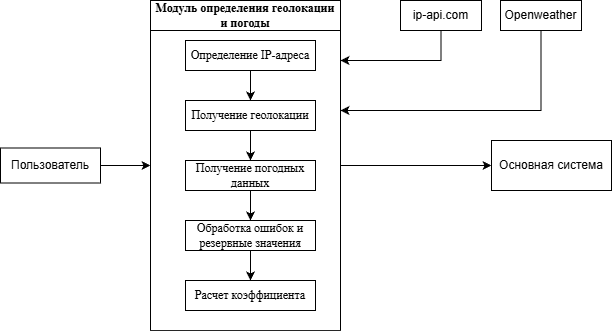
\includegraphics[width=0.9\linewidth]{pics/Picture3}
\caption{Конвейер обработки данных модуля контекстной адаптации}
\end{figure}

Процесс обработки данных включает следующие последовательные этапы:
\begin{enumerate}
    \item \textbf{Идентификация местоположения.} IP-адрес пользователя извлекается из HTTP-запроса и передаётся в RESTful API сервиса \texttt{ip-api.com}~\cite{ipapi2026}. Сервис возвращает JSON-объект, содержащий информацию о стране, регионе, городе, часовом поясе и географических координатах.
    \item \textbf{Получение метеорологических данных.} На основе полученных координат формируется GET-запрос к API \texttt{OpenWeatherMap}~\cite{openweathermap2026}, предоставляющему актуальные данные о температуре, атмосферном давлении, влажности, а также код текущего погодного условия.
    \item \textbf{Обработка ошибок и фолбэк-механизмы.} Модуль реализует трёхуровневую систему отказоустойчивости: (а) повторные запросы при временной недоступности API (retry logic с экспоненциальной задержкой); (б) использование кэшированных значений при превышении таймаута; (в) применение дефолтных региональных коэффициентов при полной недоступности внешних сервисов.
    \item \textbf{Расчёт интегрального показателя.} На основе нормализованных значений $K_{\text{region}}$, $K_{\text{temp}}$ и $K_{\text{weather}}$ вычисляется параметр~$P$ по формуле~\eqref{eq:P}, отражающий текущую предрасположенность обучающегося к эффективной учебной деятельности.
    \item \textbf{Интеграция с основной системой.} Рассчитанное значение~$P$ передаётся через сигнальный механизм Django в модуль адаптивных рекомендаций~\cite{brusilovsky2007usermodels}, где используется как весовой коэффициент при формировании персонализированной учебной траектории, выборе времени проведения аттестационных мероприятий и определении оптимальной сложности учебных материалов.
\end{enumerate}